\documentclass[12pt, oneside]{book}
\usepackage[utf8]{inputenc}
\usepackage[T1]{fontenc}
\usepackage{lmodern}
\usepackage{graphicx}
\usepackage[slovak]{babel}
\usepackage{marvosym}
\usepackage{mathtools}
\usepackage{url}            % lepsie zobrazovanie URL
\usepackage{bibentry}       % zobrazovanie celych odkazov v texte
\usepackage{tikz}
\usepackage{hyperref}
\usepackage{amsthm}
\usepackage{float}
\usetikzlibrary{shapes.geometric, arrows}
\nobibliography*            % odkazy sa maju dat aj do zoznamu literatury
\linespread{1.2}

% JAVASCRIPT DEFINITION FOR LISTING
\usepackage{listings}
\usepackage{color}
\definecolor{lightgray}{rgb}{.9,.9,.9}
\definecolor{darkgray}{rgb}{.4,.4,.4}
\definecolor{purple}{rgb}{0.65, 0.12, 0.82}

\lstdefinelanguage{JavaScript}{
  keywords={typeof, new, true, false, catch, function, return, null, catch, switch, var, if, in, while, do, else, case, break},
  keywordstyle=\color{blue}\bfseries,
  ndkeywords={class, export, boolean, throw, implements, import, this},
  ndkeywordstyle=\color{darkgray}\bfseries,
  identifierstyle=\color{black},
  sensitive=false,
  comment=[l]{//},
  morecomment=[s]{/*}{*/},
  commentstyle=\color{purple}\ttfamily,
  stringstyle=\color{red}\ttfamily,
  morestring=[b]',
  morestring=[b]"
}


\lstset{
   language=JavaScript,
   backgroundcolor=\color{lightgray},
   extendedchars=true,
   basicstyle=\footnotesize\ttfamily,
   showstringspaces=false,
   showspaces=false,
   numbers=left,
   numberstyle=\footnotesize,
   numbersep=9pt,
   tabsize=2,
   breaklines=true,
   showtabs=false,
   captionpos=b
}

\renewcommand\lstlistingname{Zdrojový kód}
% END OF JAVASCRIPT DEFINITION FOR LISTING


% -------------------
% --- Definicia zakladnych pommov
% -------------------
\def\*{{\bf FIXME: }}
\def\serviceName{SecureCloud }
\def\mfyear{2015}
\def\mftitle{Webovské rozhranie pre bezpečné zdieľanie dokumentov v cloude}
\def\mfthesistype{bakalárska práca}
\def\mfauthor{Peter Kovács}
\def\mfadvisor{RNDr. Michal Rjaško, PhD. }
\def\mfplacedate{Bratislava, \mfyear}
\def\odbor{2508 Informatika} %aj cislo odboru je povinne a je to podla katedry/odboru, na ktorom je autor
\def\program{ Informatika }
\def\stredisko{ Katedra informatiky }

\begin{document}     

% -------------------
% --- Obalka ------
% -------------------
\thispagestyle{empty}
\noindent

\begin{minipage}{0.95\textwidth}
\begin{center}
\sc  
\large
\vspace*{0.3cm} Univerzita Komenského v Bratislave\\
\vspace*{0.3cm} Fakulta matematiky, fyziky a informatiky\\
\end{center}
\end{minipage}

\vfill

\begin{minipage}{1.1\textwidth}
\begin{flushright}
\bigskip\bigskip
\center{\sc\LARGE\mftitle}
\centerline{\sc\mfthesistype}

\bigskip\bigskip\bigskip\bigskip
\end{flushright}
\end{minipage}
\vfill

\noindent \mfyear\\
\indent\mfauthor

\eject % EOP i
% --- koniec obalky ----
% -------------------
% --- Titulný list
% -------------------

\thispagestyle{empty}
\noindent

\begin{minipage}{0.95\textwidth}
\begin{center}
\sc  
\large
\vspace*{0.3cm} Univerzita Komenského v Bratislave\\
\vspace*{0.3cm} Fakulta matematiky, fyziky a informatiky\\
\end{center}
\end{minipage}

\vfill

\begin{minipage}{1.1\textwidth}
\begin{flushright}
\bigskip\bigskip
\center{\sc\LARGE\mftitle}
\centerline{\sc\mfthesistype}
\end{flushright}

\bigskip
\vspace{3cm}
\bigskip
\begin{tabular}{ll}
Študijný program: & \program \\
Študijný odbor: & \odbor \\
Školiace pracovisko: & \stredisko \\
Školiteľ: & \mfadvisor \\
\end{tabular}

\end{minipage}
\vfill

\noindent \mfplacedate\\
\indent\mfauthor

\eject % EOP i


% --- Koniec titulnej strany


% -------------------
% --- Naskenovane Zadanie
% -------------------
% v tlačenej verzii s podpismi zainteresovaných osôb.
% v elektronickej verzii sa zverejňuje zadanie bez podpisov zainteresovaných osôb.

\newpage 
\thispagestyle{empty}
\hspace{-1cm}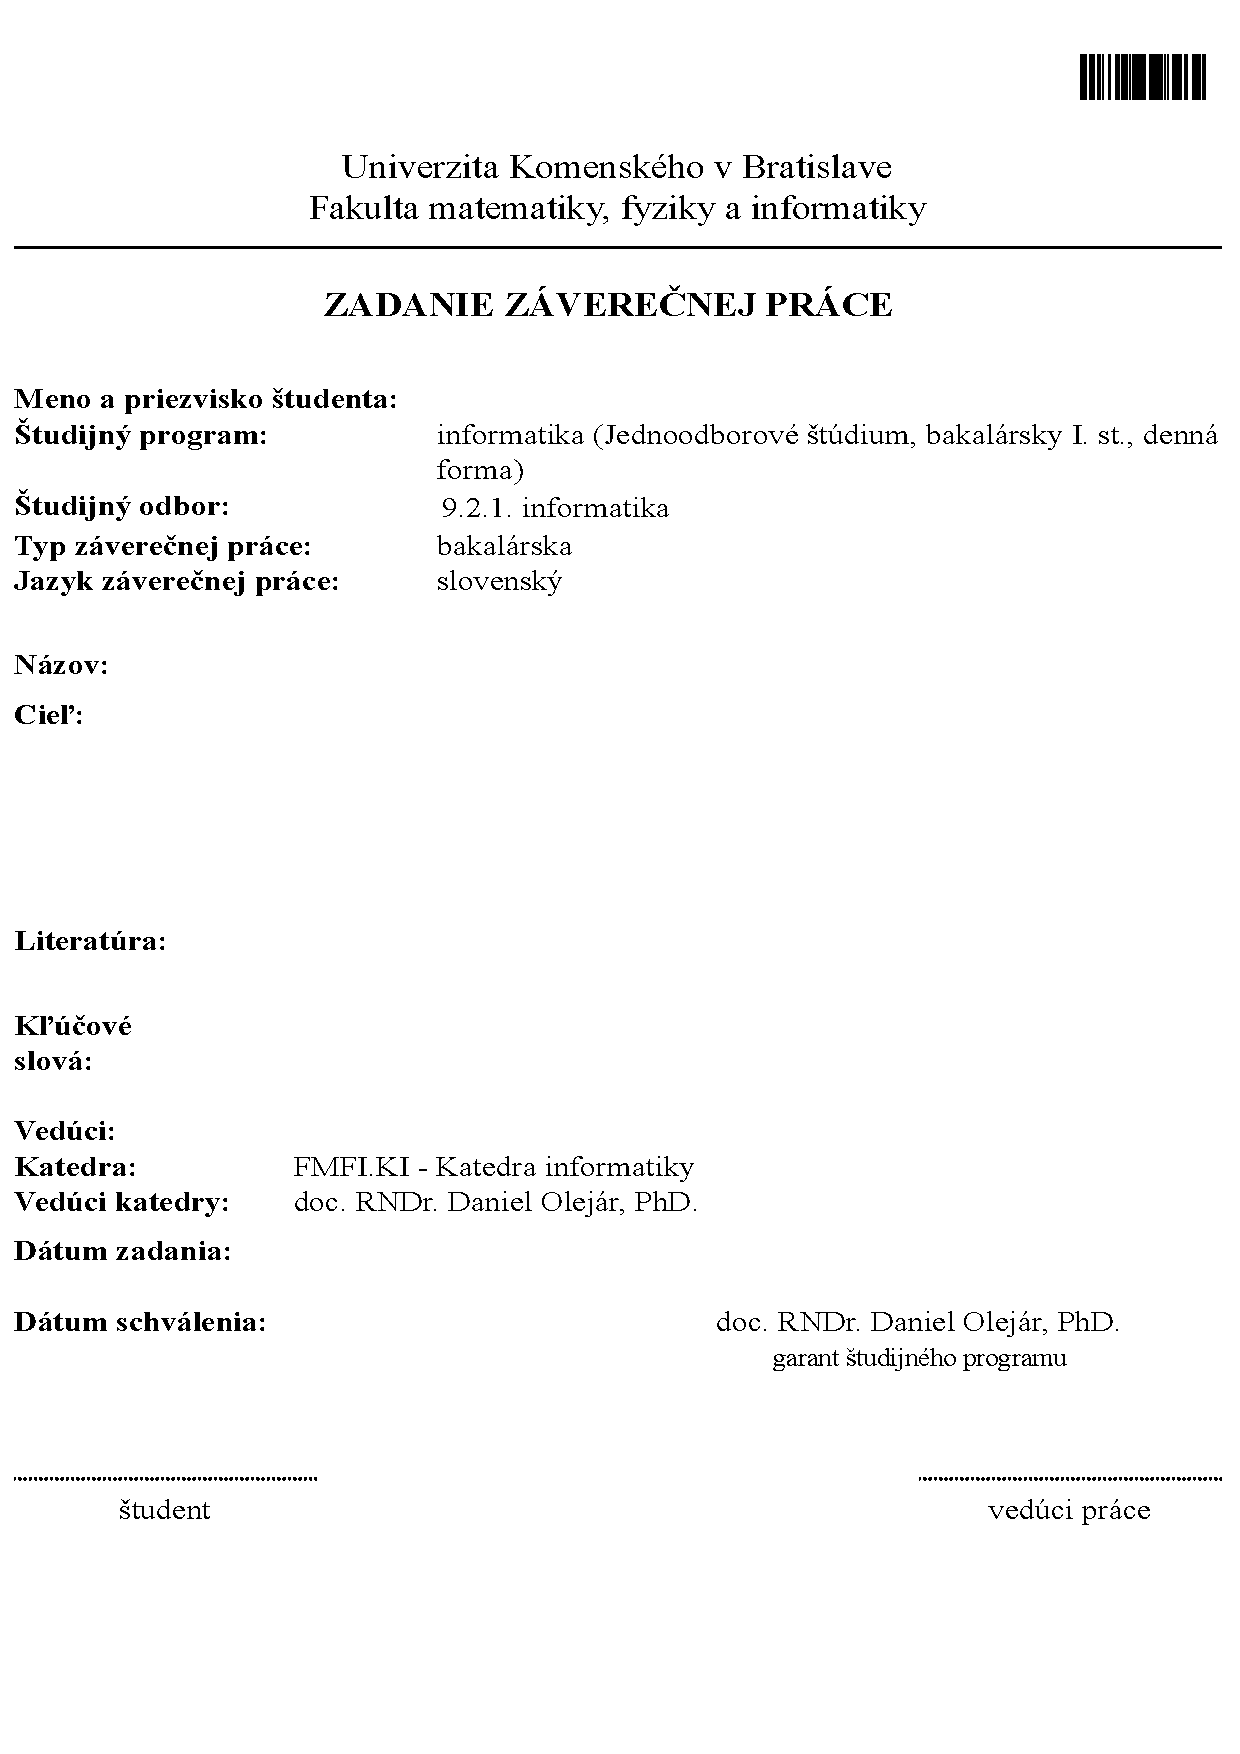
\includegraphics[width=1.2\textwidth]{images/zadanie}

% --- Koniec zadania

\frontmatter

% -------------------
%   Poďakovanie - nepovinné
% -------------------
\newpage 
\thispagestyle{empty}

\par\vspace*{\fill}
\textit{
Ďakujem RNDr. Michalovi Rjaškovi, PhD. za cenné
rady, pripomienky a odborné vedenie pri vypracovávaní
bakalárskej práce.
}

% --- Koniec poďakovania

% -------------------
%   Abstrankt - Slovensky
% -------------------
\newpage 
\thispagestyle{empty}

\huge{Abstrakt}
\normalsize
\newline
\newline
Práca sa zaoberá implementáciou webovského rozhrania, ktoré bude slúžiť na bezpečné zdieľanie dokumentov v cloude. 
Toto rozhranie tvorí vrstvu medzi cloudom a používateľom, ktorá šifruje všetky odchádzajúce dáta a dešifruje prichádzajúce.
Implementovali sme možnosť zdieľať šifrované súbory a tiež zrušenie zdieľania. Systém sme navrhli tak, aby tretia strana nemohla
získať informácie o prenášaných dátach v otvorenom tvare.
\\\\
{\bf Kľúčové slová:} web aplikácia, cloud, bezpečné zdieľanie dát
% --- Koniec Abstrakt - Slovensky


% -------------------
% --- Abstrakt - Anglicky 
% -------------------
\newpage 
\thispagestyle{empty}

\huge{Abstract}
\normalsize
\newline
\newline
The thesis focuses on an implementation of the web interface for secure file sharing in cloud. The interface is supposed to create a layer between cloud and the user which will encrypt any outgoing data and decrypt all incoming data. We have implemented functionality to share and unshare files in a secure manner. System was designed to prevent the third party from obtaining the unencrypted data.
\\\\
{\bf Keywords:} web application, cloud, secure data sharing

% --- Koniec Abstrakt - Anglicky

% -------------------
% --- Predhovor ?????
% -------------------
%\newpage 
%\thispagestyle{empty}
%
%\huge{Predhovor}
%\normalsize
%\newline
%Predhovor je všeobecná informácia o práci, obsahuje hlavnú charakteristiku práce 
%a okolnosti jej vzniku. Autor zdôvodní výber témy, stručne informuje o cieľoch 
%a význame práce, spomenie domáci a zahraničný kontext, komu je práca určená, 
%použité metódy, stav poznania; autor stručne charakterizuje svoj prístup a svoje 
%hľadisko. 
%
% --- Koniec Predhovor


% -------------------
% --- Obsah
% -------------------

\newpage 

\tableofcontents

% ---  Koniec Obsahu

% -------------------
% --- Zoznamy tabuliek, obrázkov
% -------------------

\newpage 

\listoffigures

% ---  Koniec Zoznamov

\mainmatter


\input uvod.tex 

\input kryptografia.tex

\input problem.tex

\input schema.tex

\input Implementacia.tex

\input zaver.tex

% -------------------
% --- Bibliografia
% -------------------


\newpage	

\backmatter

\thispagestyle{empty}
\nocite{*}
\clearpage

\bibliographystyle{plain}
\bibliography{literatura} 

%Prípadne môžete napísať literatúru priamo tu
\begin{thebibliography}{1}

\bibitem{HOAC} Alfred J. Menezes - Paul C. van Oorschot - Scott A. Vanstone, 1996, Handbook of Applied Cryptography, CRC Press

\bibitem{mega} Mega, Februar 2015,  [online] Dostupné na internete: https://mega.co.nz/\#doc

\bibitem{viivo} Viivo, Februar 2015,  [online] Dostupné na internete: https://viivo.com/

\bibitem{boxcryptor} BoxCryptor, Februar 2015,  [online] Dostupné na internete: https://www.boxcryptor.com/en

\bibitem{wuala} Wuala, Februar 2015, [online] Dostupné na internete: https://www.wuala.com/en/learn/technology

\bibitem{spideroak} SpiderOak, Februar 2015,  [online] Dostupné na internete: https://spideroak.com/

\bibitem{cryptree} Grolimund D. - Meisser L. - Schmid S. - Wattenhofer R., Cryptree: A Folder Tree Structure for Cryptographic File Systems, [online] Dostupné na internete: http://dcg.ethz.ch/publications/srds06.pdf
 
\bibitem{SJCLtext} Stark E. - Hamburg M. - Boneh D., Symetric Cryptography in Javascript, 2009, Annual Computer Security Applications Conference,  [online]  Dostupné na internete: https://bitwiseshiftleft.github.io/sjcl/acsac.pdf

\bibitem{SJCLgit} SJCL, Stanford Javascript Crypto Library, April 2015,  [online]  Dostupné na internete: https://github.com/bitwiseshiftleft/sjcl/

\bibitem{SJCLwiki} SJCL, Stanford Javascript Crypto Library, April 2015,  [online]  Dostupné na internete: https://github.com/bitwiseshiftleft/sjcl/wiki

\bibitem{FIPS197} NIST, Processing Standards Publication 197 - AES, April 2015,  [online]  Dostupné na internete: http://csrc.nist.gov/publications/fips/fips197/fips-197.pdf

%\bibitem{br1} MOLINA H. G. - ULLMAN J. D. - WIDOM J., 2002, Database Systems, Upper Saddle River : Prentice-Hall, 2002, 1119 s., Pearson International edition, 0-13-098043-9

%\bibitem{br2} MOLINA H. G. - ULLMAN J. D. - WIDOM J., 2000 , Databasse System implementation, New Jersey : Prentice-Hall, 2000, 653s., ???

%\bibitem{br3} ULLMAN J. D. - WIDOM J., 1997, A First Course in Database Systems, New Jersey : Prentice-Hall, 1997, 470s., 

%\bibitem{br4} PREFUSE, 2007, The Prefuse visualization toolkit,  [online] Dostupné na internete: <http://prefuse.org/>

%\bibitem{br5} PREFUSE Forum, Sourceforge - Prefuse Forum,  [online] Dostupné na internete: <http://sourceforge.net/projects/prefuse/>

\end{thebibliography}

%---koniec Referencii

% -------------------
%--- Prilohy---
% -------------------

%Nepovinná časť prílohy obsahuje materiály, ktoré neboli zaradené priamo  do textu. Každá príloha sa začína na novej strane.
%Zoznam príloh je súčasťou obsahu.
%
%\addcontentsline{toc}{chapter}{Appendix A}
%\input AppendixA.tex
%
%\addcontentsline{toc}{chapter}{Appendix B}
%\input AppendixB.tex

\end{document}






